\documentclass[10pt]{article}
\usepackage[T1]{fontenc}
\usepackage{lmodern}
\usepackage[margin=1in]{geometry}
\usepackage{amsmath,amssymb,booktabs,graphicx}
\usepackage[colorlinks=true,linkcolor=blue,urlcolor=blue,citecolor=blue]{hyperref}
\newcommand{\ParameterReduction}{11.69}
\newcommand{\ReadoutSpeedup}{1.20}
\newcommand{\MaximumParcelError}{$3.56\times10^{-8}$}

\title{Reducing TRIBE v2 Inference Cost with Affine Readout Fusion}
\author{}
\date{November 8, 2026}
\begin{document}
\maketitle
\begin{abstract}
We implement an opt-in inference rewrite of the released TRIBE v2 brain encoder
that removes an expanded intermediate readout and computes temporal averages
before the output projection. The rewrite preserves the affine map in real
arithmetic, reduces encoder parameters by \ParameterReduction\%, and provides
a \ReadoutSpeedup{}-fold measured forward speedup at batch size 8 on an AMD
Radeon RX 9070 XT. Frozen features from four HCP movies pass a float32
numerical gate for pooled and unpooled predictions. On one existing evaluation
subject, the largest absolute change in a parcel's Pearson correlation is
\MaximumParcelError. We separately evaluate pooling and attention ablations,
execution-order sensitivity, and optional compilation. These encoder measurements
exclude feature extraction; the score check is not a population equivalence study.
\end{abstract}

\section{Scope and fixed baseline}
TRIBE v2 predicts brain responses from video, audio, and language
representations~\cite{paper}. We retain its released weights, representations,
transformer, output grid, and default inference behavior. The source baseline is
commit \texttt{af58661791a351a448a489042a28f6c37e1c14b7}~\cite{code}.
The checkpoint is \texttt{best.ckpt} at Hugging Face revision
\texttt{f894e783020944dcd96e5568550afe2aa9743f9f}~\cite{weights}.

The encoder receives 200 input steps, with two feature groups per modality and
widths 3072 (text), 1024 (audio), and 1408 (video). It uses hidden width $H=1152$,
eight transformer layers, and intermediate readout width $R=2048$, producing
$O=20484$ cortical values at 100 output steps. Although named
\texttt{low\_rank\_head}, the released intermediate projection expands the hidden
width. The output predictor contains one shared subject row; our rewrite does
not introduce averaging over a subject bank.

\section{Inference rewrite}
For hidden state $h_t\in\mathbb{R}^{H}$, bias-free intermediate projection
$W\in\mathbb{R}^{R\times H}$, shared output weights
$A\in\mathbb{R}^{O\times R}$, and bias $b\in\mathbb{R}^{O}$,
\begin{equation}
y_t=AWh_t+b=Ch_t+b,\qquad C=AW\in\mathbb{R}^{O\times H}.
\label{eq:fusion}
\end{equation}
There is no nonlinearity between these projections. Storing $C$ eliminates
$RH+OR-OH=20{,}712{,}960$ parameters without changing the real-arithmetic map.
Composition runs once on the CPU in float64 and is cast to the original dtype;
inference remains float32.

Adaptive average pooling from $T$ to $T'$ steps uses bins~\cite{pooling}
\begin{equation}
S_j=\{t:\lfloor jT/T'\rfloor\leq t<\lceil(j+1)T/T'\rceil\},
\quad j=0,\ldots,T'-1.
\end{equation}
Because each bin's averaging weights sum to one,
\begin{equation}
\frac{1}{|S_j|}\sum_{t\in S_j}(Ch_t+b)
=C\left(\frac{1}{|S_j|}\sum_{t\in S_j}h_t\right)+b.
\label{eq:pool}
\end{equation}
We therefore pool hidden states before applying $C$. This also holds for unequal
or overlapping bins and for upsampling. With \texttt{pool\_outputs=False},
pooling is omitted. Floating-point evaluation orders differ, so bitwise equality
is not assumed.

\subsection{Compatibility boundaries}
\texttt{TribeModel.from\_pretrained(..., optimize=True)} converts on the CPU
before device transfer; the default is \texttt{False}. An already loaded
evaluation-mode model can also be converted in place. Conversion requires the
shared predictor with \texttt{average\_subjects=True} and nonzero
\texttt{subject\_dropout}, as required by the dependency. Without an
intermediate projection, the selected shared row is cloned to release unused
subject storage.

Conversion is inference-only and idempotent. Calling \texttt{train()} afterwards
raises an error. The changed weight shapes and removed intermediate layer make
the converted state dictionary incompatible with the original configuration;
reload the original checkpoint and convert again. The original path retains
strict checkpoint loading and backpropagation. Research code extracting the
original 2048-dimensional representation must keep the unconverted model.

\section{Evaluation}
\subsection{Inputs and fidelity}
We use 40 frozen, 100-second feature windows, ten per movie. The movies are
\texttt{MOVIE1\_CC1}, \texttt{MOVIE2\_HO1}, \texttt{MOVIE3\_CC2}, and
\texttt{MOVIE4\_HO2}, in that order. Valid lengths are 921, 918, 915, and 901
output steps. Read-only cache preparation reproduces every evaluated input tensor
exactly. Raw inputs, recordings, subject identifiers, and checkpoints remain local.

Original and candidate outputs use identical runtime, device, dtype, and inputs.
The elementwise gate is $|\hat y-y|\leq10^{-5}+10^{-4}|y|$, with finite
outputs required. We record maximum absolute and relative $\ell_2$ errors.
Global output correlation is only a numerical diagnostic. Pooled and unpooled
predictions are checked separately on all movies. Original timelines agree with
the existing saved predictions within the same gate; trailing padding is removed.

One previously evaluated HCP subject supplies a score regression check under
the existing HCP-native 2025 preprocessing. The canonical fixed lag is $-5$:
predictions at $0,\ldots,n-6$ are compared with BOLD at $5,\ldots,n-1$.
There is no lag search. We average vertices within each of 360 labeled parcels,
compute each parcel's temporal Pearson correlation, and average those
correlations. Labeled-vertex mean squared error (MSE) is separate.
Numerical score gates require absolute changes below $10^{-6}$ in both mean
and maximum parcel correlation and absolute relative MSE change below $10^{-5}$.
The maximum-parcel gate was added during review to prevent cancellation.
These are regression gates, not statistical equivalence margins. No model
is trained or selected using this subject's brain scores.

\subsection{Runtime and alternatives}
Accelerator measurements use an AMD Radeon RX 9070 XT (16 GB), PyTorch
\texttt{2.12.0+rocm7.14.0}, and HIP \texttt{7.14.60850}. CPU measurements use
an Intel Core i5-13500, four intra-op threads, and PyTorch \texttt{2.6.0+cpu}.
Python is 3.12; \texttt{neuraltrain} and \texttt{neuralset} are 0.0.2,
\texttt{x-transformers} is 1.27.20, and NumPy is 2.2.6. ROCm is outside the
upstream Torch $<2.7$ constraint, so CPU compatibility is checked separately.
This is not a clean-install test of all optional dependencies or a test of NVIDIA.

Each condition uses a fresh model and identical batch sequence. After warm-up,
forward wall time is measured with accelerator synchronization around every call.
GPU batch 1 uses 80 calls and 10 warm-ups; GPU batch 8 uses 60 and 10;
CPU batch 1 uses 40 and 5. Transfers and cache I/O are outside the timer.
Intervals are empirical interquartile ranges, not confidence intervals.
Batch-8 measurements are repeated in reverse condition order.

Conditions are baseline, pooling only, fused readout with early pooling, SDPA
only, and fused readout plus SDPA. SDPA uses the dependency's existing PyTorch
scaled-dot-product attention path; its name does not establish the kernel selected.
Allocated-memory peaks include input tensors and differ from physical VRAM,
reserved memory, and activation-only costs. Conversion time and process RSS
sampled every 5 ms are separate; brief RSS peaks can be missed. In-place
conversion includes the original device model and does not measure cold loader
peak memory.

Optional \texttt{torch.compile} is a separate comparison against fused eager
inference. All frozen batches are checked before steady timing. First-call
times include existing compiler-cache effects, not clean-cache compilation.
Its order is fixed (eager then compiled), so the observed ratio is exploratory.
Compilation is not adopted for the four-movie workload: its seconds of startup
cost exceed the tens of milliseconds saved in steady inference.

\section{Results}
The encoder parameter count decreases from 177,205,397 to 156,492,437 (11.69\%). Float32 parameter storage decreases from 675.98 to 596.97 MiB. Table~\ref{tab:runtime} reports forward latency; each runtime is a separate comparison.

\begin{table}[htbp]\centering\sffamily\small
\caption{Median forward latency (ms) and baseline/fused speed ratio}\label{tab:runtime}
\begin{tabular}{@{}lrrrr@{}}\toprule
Runtime & Baseline & Fused & Fused + SDPA & Ratio \\\midrule
ROCm, batch 1 & 11.31 & 10.22 & 11.16 & 1.11 \\
ROCm, batch 8 & 42.91 & 35.69 & 40.03 & 1.20 \\
CPU Torch 2.6, batch 1 & 163.67 & 133.47 & 133.37 & 1.23 \\
\bottomrule\end{tabular}\end{table}

Table~\ref{tab:ablation} separates the candidate changes on ROCm at batch 8. The intervals are sample quartiles, not confidence intervals. Allocator peaks include input tensors; they are not physical VRAM or activation-only measurements.

\begin{table}[htbp]\centering\sffamily\small
\caption{ROCm batch-8 ablation and peak tensor allocation}\label{tab:ablation}
\begin{tabular}{@{}lrrr@{}}\toprule
Variant & Median (ms) & IQR (ms) & Peak (MiB) \\\midrule
Baseline & 42.91 & [42.83, 43.02] & 1010.19 \\
Pooling only & 37.78 & [37.69, 37.88] & 999.94 \\
Fused readout & 35.69 & [35.59, 35.74] & 919.85 \\
SDPA only & 47.35 & [47.25, 47.44] & 1010.19 \\
Fused + SDPA & 40.03 & [39.96, 40.11] & 854.23 \\
\bottomrule\end{tabular}\end{table}

In-place batch-8 conversion takes 553.03 ms. Its sampled incremental process RSS is 533.80 MiB and its peak GPU tensor allocation is 843.20 MiB. Dividing this conversion time by the observed per-call saving gives about 77 batch-8 calls to amortize conversion. This is an in-place estimate, not a cold-loader measurement. A single four-movie pass has only five batch-8 calls, so a total-runtime benefit is not established for that workload. Parameter savings apply immediately; forward-time savings favor reusing the converted model.

Table~\ref{tab:fidelity} reports the existing-subject regression check. All four movies pass pooled and unpooled numerical gates.

\begin{table}[htbp]\centering\sffamily\small
\caption{Mean parcel correlation and numerical differences for one existing evaluation subject}\label{tab:fidelity}
\begin{tabular}{@{}lrrrr@{}}\toprule
Movie & Baseline $r$ & Fused $r$ & $\Delta$ mean $r$ & Max parcel $|\Delta r|$ \\\midrule
1 & 0.236518 & 0.236518 & $1.49\times10^{-10}$ & $2.98\times10^{-8}$ \\
2 & 0.263297 & 0.263297 & $-5.81\times10^{-10}$ & $2.90\times10^{-8}$ \\
3 & 0.200522 & 0.200522 & $-1.29\times10^{-9}$ & $3.30\times10^{-8}$ \\
4 & 0.257067 & 0.257067 & $-3.68\times10^{-10}$ & $3.56\times10^{-8}$ \\
\bottomrule\end{tabular}\end{table}

The largest pooled and unpooled absolute prediction differences are $4.77\times10^{-6}$ and $5.60\times10^{-6}$, respectively. The largest absolute relative change in labeled-vertex MSE is $2.68\times10^{-10}$. No population-level equivalence test is claimed.

In the separate batch-1 compiler experiment, fused eager inference takes 10.19 ms and compiled inference 8.89 ms (observed timing ratio 1.15). The first compiled call takes 1.92 s with the existing compiler cache; this is not a clean-cache compilation estimate.

In the separate batch-8 compiler experiment, fused eager inference takes 35.49 ms and compiled inference 32.00 ms (observed timing ratio 1.11). The first compiled call takes 8.15 s with the existing compiler cache; this is not a clean-cache compilation estimate.

With the condition order reversed at batch 8, baseline and fused medians are 48.68 and 41.30 ms, respectively (ratio 1.18).

Figures~\ref{fig:performance} and~\ref{fig:fidelity} display the runtime and
numerical regression measurements.
\begin{figure}[htbp]
\centering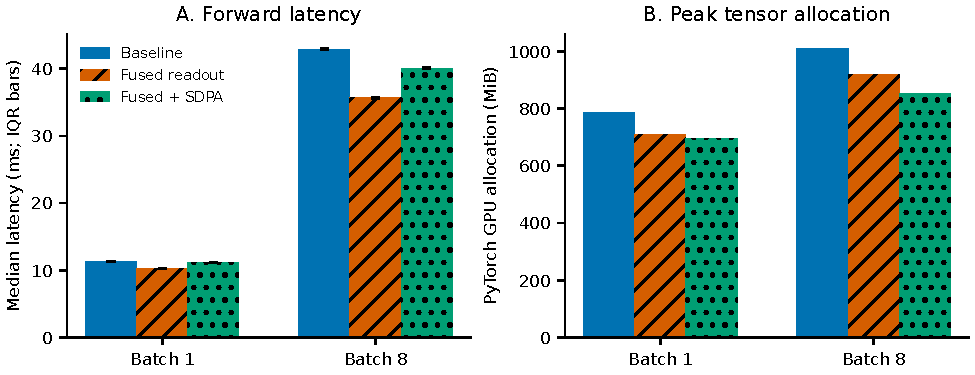
\includegraphics[width=\linewidth]{performance.pdf}
\caption{ROCm forward latency and peak tensor allocation with identical frozen
inputs. Color and pattern distinguish the three conditions. Error bars mark
sample quartiles. Timing excludes feature extraction and host-to-device transfer;
memory is PyTorch allocation, not physical VRAM.}
\label{fig:performance}
\end{figure}
\begin{figure}[htbp]
\centering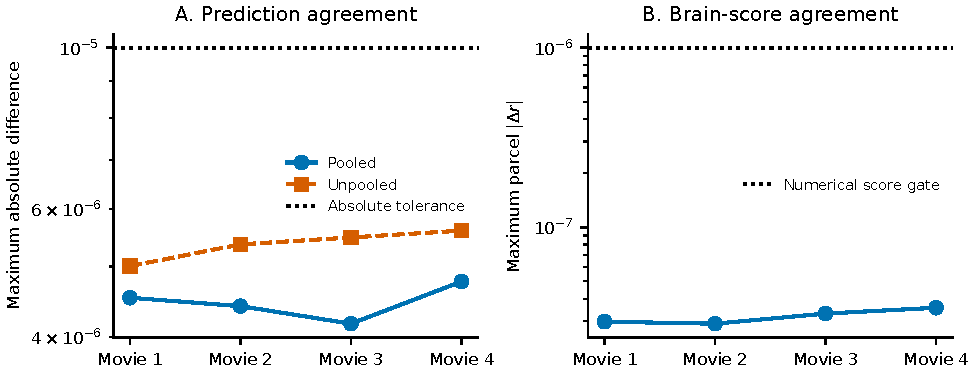
\includegraphics[width=\linewidth]{fidelity.pdf}
\caption{Numerical differences for the four movies in the order stated above.
Left: maximum pooled and unpooled prediction differences; the dotted line is
the absolute part of the combined tolerance. Right: maximum absolute parcel
correlation change for one existing subject and its numerical score gate.
Both vertical axes are logarithmic. No population uncertainty is implied.}
\label{fig:fidelity}
\end{figure}

\section{Decision and limitations}
The opt-in fused readout reduces parameters and measured forward cost while
passing the tested numerical and score gates. Its algebraic basis does not
depend on these movies, but floating-point behavior has only been tested under
the stated conditions. The one-time fusion cost must be amortized when runtime
is the objective; the measurements do not establish a cold-start benefit for a
single short pass. SDPA changes the speed--memory tradeoff and remains an
experimental condition rather than being silently enabled. Compilation is
optional because startup cost can exceed the savings for a short run.

The rewrite does not reduce the pretrained stimulus extractors or the original
checkpoint's disk size. Pruning, quantization, alternative extractors, and
retraining require separate validation. One subject cannot establish population
or out-of-distribution equivalence. Clock and workload variability limit latency
extrapolation. The review and experiments resolve the tested candidates; they
do not prove that future optimization is impossible.

\section{Reproduction and review}
The repository includes cache preparation, inference and compiler benchmarks,
the fixed-lag evaluator, aggregate JSON, and \texttt{benchmarks/render\_report.py},
which regenerates tables and figures. Real-input experiments require the original
checkpoint and licensed local data; synthetic benchmarking is also available.
The experiment record and review log document decisions.

DeepSeek V4.1 Flash produced implementation, benchmark, and report drafts through
OpenCode Go. Codex inspected and corrected them, ran experiments, and coordinated
independent review. Tests cover checkpoint round trips, backpropagation, shared
row selection, storage release, unequal pooling, unpooled outputs, and
inference-only boundaries. The derivative retains CC-BY-NC-4.0 and attribution.

\begin{thebibliography}{9}
\bibitem{paper} S. d'Ascoli et al. \emph{A foundation model of vision, audition,
and language for in-silico neuroscience}. arXiv:2605.04326, 2026.
\url{https://arxiv.org/abs/2605.04326}.
\bibitem{code} Meta Platforms, Inc. \emph{TRIBE v2 source code}.
\url{https://github.com/facebookresearch/tribev2}.
\bibitem{weights} Meta Platforms, Inc. \emph{TRIBE v2 released weights}.
\url{https://huggingface.co/facebook/tribev2}.
\bibitem{pooling} PyTorch contributors. \emph{Adaptive pooling index definitions},
version 2.6.0, \texttt{AdaptivePooling.h}.
\href{https://github.com/pytorch/pytorch/blob/v2.6.0/aten/src/ATen/native/AdaptivePooling.h}{Source file on GitHub}.
\end{thebibliography}
\end{document}
